\chapter{Implementation}
\section{The use of frameworks}
Using frameworks because of the decreased development time due to already developed and tested libraries for various tasks such as database accesss, file handling and file uploading.

\section{Backend}
\subsection{The C++ application}
\subsubsection{Why a C++ application?}
We're using a C++ application because it is much faster to parse huge files in C++ than PHP or JavaScript.
The choice of language was because we had some knowledge of both C and C++. C++ is object oriented where as C is a procedural language, and seeing as we all favour object oriented programming, the choice between the two was easy.

We could have chosen other languages such as F, F\#, Java, Perl or Ruby, but our limited knowledge about these made us stick with C++, which is also quite fast and portable.

\subsubsection{Why Qt?}
We've decided to use Qt because of the support and community around it. It's very mature and most importantly, object oriented.

Qt is a cross-platform application framework developed by Nokia. Popular software such as Skype, VLC media player and VirtualBox along with companies as Google, HP, Philips and Samsung uses it.

Qt makes developing an application with a GUI\footnote{Graphical User Interface} relatively easy, but we've opted to only use the command line part of Qt, because the programming is run by the application and not by a user.

\subsubsection{Return codes}
The PHP part of the application gets a return code from the C++ application depending on how the parsing went and reacts accordingly. A list of the return codes can be seen in table \ref{tab:cppReturnCodes}.
\begin{table}[htbp]
\centering
\begin{tabular}{|l|l|}
\hline
\textbf{Code} & \textbf{Explanation}\\
\hline
0 & Failure\\
\hline
1 & Success\\
\hline
2 & Success, unkown params ignored\\
\hline
10 & Failed, missing fileid\\
\hline
11 & Failed, missing filename\\
\hline
12 & Failed, missing type\\
\hline
20 & Unknown file type\\
\hline
21 & File not found\\
\hline
22 & Invalid file, or wrongly formatted\\
\hline
30 & Could not read input file\\
\hline
31 & Could not write to input file\\
\hline
32 & Could not read output file\\
\hline
33 & Could not write to output file\\
\hline
34 & Could not delete output file\\
\hline
\end{tabular}
\caption{Return codes from the C++ application}
\label{tab:cppReturnCodes}
\end{table}

\subsubsection{Extensibility}
The application is coded with extensibility in mind, and all parsers is therefore extending the base class \emph{Parser}.
The \emph{Parser} class contains the basic methods of setting the filename, opening for read and write and closing the open file handle.\todo[color=red,fancyline]{Explain more in-depth?}

\subsection{The PHP site}
\subsubsection{Why PHP?}

\subsubsection{Why FuelPHP?}

\subsubsection{Speed optimizations}
At the beginning the chart had monthly, weekly and daily view, but when loading all data for one month, the performance were so poor. This was fixed by changing views to 2-weekly, weekly and daily view.

\subsubsection{Caching}
Caching has been implemented both server and client side, to allow for maximum performance when viewing charts and radar image animations.

\begin{table}[htbp]
\centering
\begin{tabular}{|l|l|l|l|}
\hline
\textbf{Area} & \textbf{Before} & \textbf{Server side} & \textbf{Server + client side}\\
\hline
Radar & \textasciitilde 130-150 ms & \textasciitilde 35 ms & \textasciitilde 2 ms\\
\hline
Chart & \textasciitilde 300 ms & \textasciitilde 40 ms & \textasciitilde 2 ms\\
\hline
\end{tabular}
\label{tab:cache_benchmarks}
\caption{Cache benchmarks}
\end{table}

When a radar image or chart data is requested, the server checks if a cache of the output exists. If it does, it checks if the browser already have a copy of the same cache file and send a \textsf{301 Not Modified} response to the browser, telling it to its own file.
If the browser does not have a cache, or it is too old, the server sends the contents of the new cache to the browser.
If no cache is found on the server, or it has expired, the server retrieves the needed info from the database, generate the image or data to output, saves it to the cache and sends it to the browser.


\subsubsection{The data}
The application support the upload of the following file types:
\begin{description}
\item[csv] Observations form a wind farm. The definition can be found in appendix \ref{ap:csv}.
\item[wrk] Weather image from a radar. The file must obey the new VRIS format. See \cite{VRIS} for the definition of VRIS.
\item[zip] All supported file formats can be zipped to easily upload multiple files at the same time. Unlimited zip and folder nesting is supported\footnote{Note that there might be a limit on the file- or foldername length set by the operating system.}.
\end{description}

\section{Frontend}
\subsection{jQuery}
\todo[inline]{Quick roundup about the use of jQuery}
There has been used JavaScript\footnote{Client-side scripting language for web pages} to load and visualize data. It gives a more smooth design, since the pages don't have to reload every time, but can be loaded in background.

The JavaScript framework there has been used is jQuery\footnote{JavaScript framework, see \cite{jquery} for the documentation}, because of the very well documentation. jQuery is one of the most popular JavaScript library and is free open source software. The animations for map and chart are made by using jQuery.
 
One of the techniques with jQuery is for instance AJAX\footnote{Asynchronous JavaScript and XML}, which enables the chart to send data to, and retrieve data from, the server asynchronously. Data is retrieved using XMLHttpRequest, since the data is ready in JSON\footnote{JavaScript Object Notation - representing simple data structures and associative arrays}.

If the browser doesn't support JavaScript or it isn't up-to-date, the user still have access to upload files, but not viewing data from map or chart.

\subsection{Bootstrap}
\todo[inline]{Quick roundup about the use of Boostrap and its support for smartphones and tablets}
Today many people keep them updated on the fly and to give them the opportunity, we have tried to create a design that also works on smartphones, that have smaller screens and lesser processing power. Most of the calculating is done on the server, so the requirements for client-side is almost nothing, other than showing the data that the server has performed.

The only problem with smartphone is the smaller screen, sometimes it can be difficult to get a good look, specially the charts are a problem.

We have tried accessing the software with iPhone and Android. On the iPhone the only problem was the chart, because you couldn't see the whole chart. Radar and map were working just fine, like on a normal PC.

\section{Cross-platform compability}
\label{sec:cross-platform}
The use of PHP, C++ and MySQL allows the execution of the application on almost all platforms, because the technologies used are open source and available on most platforms.

We have, however, chosen to drop support for all version of Internet Explorer, because this would increase development time drastically -- time we did not have.

% db.tex should start at section level
\section{Database}
\label{sec:database}
All tables will contain an \textsf{id} column, such that all rows in the same table are unique. This also makes it easy to fetch and perform actions for a specific row.

\textsf{users} table should at minimum contain the columns \textsf{username, password} and \textsf{email}.

\textsf{files} table should at minimum contain the columns \textsf{name, latitude, longitude, path, type} and \textsf{offset}.
Also, as it would be convenient to know who uploaded the file, a \textsf{user\_id} field should also be created.

There will be a table for all supported file types (currently \textsf{csv} and \textsf{wrk}). \textsf{csv} table should contain columns as stated in appendix \ref{ap:csv}, and \textsf{wrk} as defined by the VRIS\footnote{See \cite{VRIS} for definition} file format. Besides these columns, all file type tables should contain a \textsf{file\_id} field so all data is related to the source file (in the database).

As the database should be able to handle a large amount of data, it is crucial that all columns are of correct and optimal data types, e.g. \textsf{id} columns are either \textit{int} or \textsf{bigint} and are \textsf{unsigned}. By comparison, \textsf{unsigned int} can take the maximum value $2^{32}-1 (\approx 4.29 \cdot 10^{9})$ while it for \textsf{unsigned bigint} is $ 2^{64}-1 (\approx 18.45 \cdot 10^{18})$.

Figure \ref{fig:dbdiagram} is a diagram of the database has been implemented based on the analysis and design.

\begin{figure}[htbp]
   \centering
   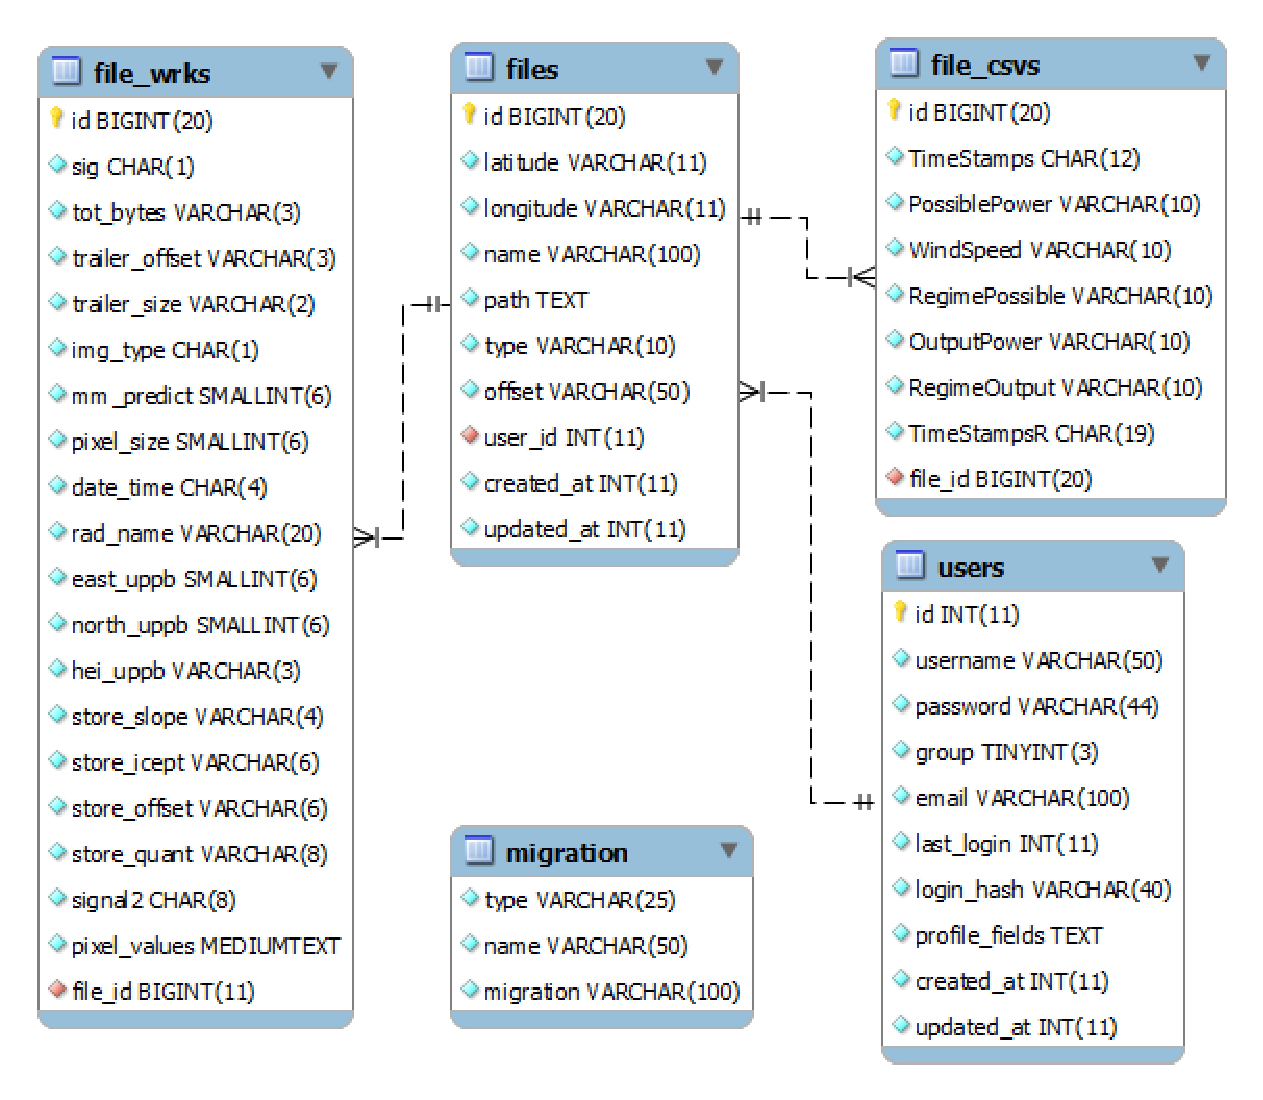
\includegraphics[width=1\linewidth]{figure/db}
   \caption{Database Diagram}
   \label{fig:dbdiagram}
\end{figure}

FuelPHP contains a \textsf{migration} tool that lets one create revisions for the database, hence easy deployment of changes. This tool has been used to create all tables, and therefore the \textsf{migration} table is used to keep track of revisions.

All tables use \textsf{InnoDB}, because this engine make it possible to create sql relations. This means that if a table has a foreign key (i.e. a key that identifies a row in another table), one can create actions for what should happen to the rows in the current table, if the related row in the other table is \textsf{updated} or \textsf{deleted}.

These relations can be seen in the diagram. The relations and actions is stated by sql as in listing \ref{lst:sql}
\begin{lstlisting}[language=sql,caption={SQL realations and actions},label={lst:sql}]
ALTER TABLE `files`
  ADD CONSTRAINT `files_ibfk_1` FOREIGN KEY (`user_id`) REFERENCES `users` (`id`) ON DELETE NO ACTION ON UPDATE NO ACTION;

ALTER TABLE `file_csvs`
  ADD CONSTRAINT `file_csvs_ibfk_1` FOREIGN KEY (`file_id`) REFERENCES `files` (`id`) ON DELETE CASCADE ON UPDATE NO ACTION;

ALTER TABLE `file_wrks`
  ADD CONSTRAINT `file_wrks_ibfk_1` FOREIGN KEY (`file_id`) REFERENCES `files` (`id`) ON DELETE CASCADE ON UPDATE NO ACTION;
\end{lstlisting}

\subsection{Optimization}
\label{sec:database_optimization}
In FuelPHP it is possible to create model relations that are similar to sql relations with actions, but easier to manage and at the same time less efficient (though generally adequate). This method was used initially, but performance was found to be too bad, e.g. it would take too much time to cascade delete all the csv rows related to the file selected for deletion, eventually leading to a time out by the server. The time out limit can be changed by the server manager, but it was easier and - as stated before - more efficient to make relation actions in sql. Relations are still present at model level, but actions have been turned off.

When first creating the database, the data types for the fields were not optimized, and as previously stated this is important for performance, and improper data types or constraints can even break the data that should be saved. When optimising the data types, we were also able to gain space and e.g. halve the size of the \textsf{file\_csvs} from maximum 372 bytes per row to maximum 107 bytes.

As seen on figure \ref{fig:dbdiagram}, \textsf{id} for  \textsf{files, file\_csvs} and  \textsf{file\_wrks} are of type \textsf{bigint} ( \textsf{unsigned}). This make it possible for these tables to store a huge amount of data, and even though \textsf{unsigned int} can save a large amount too, we would rather make the application future proof than let it break if the limit was reached.

Equations \ref{eq:db_1} through \ref{eq:db_4} illustrate the problem and reason for the decision made.

\emph{Number of csv files stored, if the data is represented by a 10 minute interval in a span of 1.5 years (as current test data):}

\textsf{unsigned int}: 
\begin{equation}
\label{eq:db_1}
\left\lfloor \frac{2^{32}-1}{72,858} \right\rfloor = 58,949
\end{equation}

\textsf{unsigned bigint}:
\begin{equation}
\label{eq:db_2}
\left\lfloor \frac{2^{64}-1}{72,858} \right\rfloor = 253,187,626,255,312
\end{equation}

\emph{Number of csv files stored, if the data is represented by a 1 minute interval in a span of 1.5 years:}

\textsf{unsigned int}:
\begin{equation}
\label{eq:db_3}
\left\lfloor \frac{2^{32}-1}{72,858 \cdot 10} \right\rfloor = 5,894
\end{equation}

\textsf{unsigned bigint}:
\begin{equation}
\label{eq:db_4}
\left\lfloor \frac{2^{64}-1}{72,858 \cdot 10} \right\rfloor = 25,318,762,625,531
\end{equation}

As the storage size of \textsf{bigint} is only twice as big as \textsf{int}, the maximum increase in storage per row is not remarkable, where as the increase in number of possible files storeable is increased by a huge margin as seen on equation \ref{eq:db_3} and \ref{eq:db_4}.

% api.tex should start at section level
\section{API}
The application has a small API\footnote{Application programming interface} that the application it self uses to retrieve some of the data.

\subsection{Radars}
A list of images for a radar can be retrieved by calling
\begin{lstlisting}[language=sh]
GET http://WEBROOT/rest/radar/list.TYPE?lat=LAT&lng=LNG&f=FROM
\end{lstlisting}
Where \textsf{WEBROOT} is the domain name of the server, \text{TYPE} is the return type\footnote{All formats supported by FuelPHPs REST controller is supported. A list of supported formats can be found at \url{http://docs.fuelphp.com/general/controllers/rest.html\#/formats}.\label{fn:fuel_rest}}, \textsf{LAT} is the latitude of the radar, \textsf{LNG} is the longitude of the radar and \text{FROM} is a date from which the data should start from.

The returned data is in array format, where each element is an array consisting of two elements. The first is the timestamp of the image, and the second is the url of the radar image relative to the \textsf{WEBROOT}.

\subsection{Wind farms}
A list of data from a given wind farm can be retrieved by calling
\begin{lstlisting}[language=sh]
GET http://WEBROOT/rest/csv/list.TYPE?id=ID&c=COL&f=FROM&t=TO
\end{lstlisting}
Where \textsf{WEBROOT} is the domain name of the server, \textsf{TYPE} is the return type\footref{fn:fuel_rest}, \textsf{ID} is ID of the wind farm, \textsf{COL} is the column\footnote{Currently \textsf{PossiblePower}, \textsf{OutputPower}, \textsf{WindSpeed}, \textsf{RegimePossible} and \textsf{OutputRegime}. Note that the columns are case-sensitive.} to fetch data from, \text{FROM} is a date from which the data should start from and \text{TO} is a date at which the data stops at.

The returned data is in array format, where each element is an array consisting of two elements. The first is the timestamp of the image, and the second is the url of the radar image relative to the \textsf{WEBROOT}.

\subsection{Jobs}
A number of files currently in queue to be parsed can be retrieved by calling
\begin{lstlisting}[language=sh]
GET http://WEBROOT/rest/jobs/list.TYPE
\end{lstlisting}
Where \textsf{WEBROOT} is the domain name of the server.

\subsection{Upload}
It is possible to send data to the application, just as if they were being uploaded manually. This allows for remote services to send `real time' data to the application. To send data to the server, the following call should be made:
\begin{lstlisting}[language=sh]
curl -F "path=@FILE" http://WEBROOT/api/upload -H "X-KEY: KEY=" -H "X-TIMEZONE: ZONE" -X POST
\end{lstlisting}
Where \textsf{FILE} is the path to the file on the senders machine, \textsf{WEBROOT} is the domain name of the server, \textsf{KEY} is an API key and \textsf{ZONE} is the time zone given by MySQLs Zoneinfo\footnote{See section \ref{sec:application_requirements} for notes about installation of Zoneinfo}.

An example call, to upload \textsf{ekxr20101218\_2350.wrk} with UTC timestamps to the \textsf{WEBROOT} server with the default admin user woudl look like this:
\begin{lstlisting}[language=sh]
curl -F "path=@ekxr20101218_2350.wrk" http://WEBROOT/api/upload -H "X-KEY: YWqmPGH+dOEvOh6pf83a62lzJ1QQLHRMPHhNIaohB3s=" -H "X-TIMEZONE: UTC" -X POST
\end{lstlisting}

